\documentclass[11pt]{article}
\usepackage[utf8]{inputenc}
\usepackage[T1]{fontenc}
\usepackage{amsmath}
\usepackage{amsfonts}
\usepackage{geometry}
\usepackage{hyperref}
\usepackage{titlesec}
\usepackage{graphicx}
\usepackage{float}
\usepackage{booktabs}
\usepackage{multicol}
\usepackage{enumitem}
\usepackage{subcaption}

\geometry{a4paper, margin=0.85in}

\titleformat{\section}{\large\bfseries}{}{0em}{}[\titlerule]
\titleformat{\subsection}{\bfseries}{}{0em}{}
\setlength{\parskip}{3pt}
\setlength{\parindent}{0pt}

\begin{document}

% --- TITLE PAGE ---
\begin{titlepage}
	\centering
	\vspace*{2cm}
	\Huge\textbf{IKT215 Final Project: \\ Fashion MNIST Classification \\ Dense Neural Networks vs. kNN} \\
	\vspace{1.5cm}
	\Large \textbf{Student:} Gomery K. Wanjiru \\
	\Large \textbf{Course:} IKT215 -- Pattern Recognition \\
	\Large \textbf{Date:} May 2026 \\
	\vfill
	\section*{Disclaimer on Generative AI}
	In accordance with UiA's guidelines, I declare that I used Generative AI tools (GitHub Copilot / Claude) to assist in structuring the LaTeX report layout, generating boilerplate plotting code, and parallelizing the kNN cross-validation with joblib. The experimental design, hyperparameter selection rationale, neural network architecture choices, interpretation of results, and comparative analysis are my own work, guided by the course lecture materials (Lectures 1--12) and exercises.
\end{titlepage}

\newpage
\section{Introduction}

This project evaluates two classification approaches on the Fashion MNIST dataset: the k-Nearest Neighbors (kNN) algorithm as a non-parametric baseline and dense (fully connected) neural networks as a parametric, learned representation approach. The goal is to compare their performance and analyze their relative strengths and weaknesses for image classification.

Fashion MNIST \cite{xiao2017} is a drop-in replacement for the original MNIST digit dataset, containing 70,000 grayscale images of clothing items across 10 classes. It is intentionally more challenging than digit MNIST, making it a suitable benchmark for evaluating classification methods.

\subsection{Problem Statement}
Given 28$\times$28 grayscale images of clothing items, classify each image into one of 10 categories: T-shirt/top, Trouser, Pullover, Dress, Coat, Sandal, Shirt, Sneaker, Bag, and Ankle boot. We investigate:
\begin{enumerate}[nosep]
	\item How well does kNN perform with optimal hyperparameters?
	\item Does PCA dimensionality reduction improve kNN efficiency without sacrificing accuracy?
	\item Can a dense neural network learn better representations and outperform kNN?
	\item What classes are most difficult, and why?
\end{enumerate}

\section{Methodology}

\subsection{Data Preprocessing}
The dataset consists of 60,000 training and 10,000 test images. Each 28$\times$28 image is flattened into a 784-dimensional vector. Pixel values are normalized from $[0, 255]$ to $[0, 1]$ by dividing by 255. This normalization is critical for:
\begin{itemize}[nosep]
	\item \textbf{kNN}: Distance metrics (Euclidean, Manhattan) are sensitive to feature scale; normalizing ensures all pixels contribute equally.
	\item \textbf{Neural networks}: Inputs in $[0, 1]$ prevent large activations and improve gradient flow during training.
\end{itemize}
The dataset is perfectly balanced (6,000 samples per class in training, 1,000 per class in test), so no class weighting or resampling is required.

\subsection{kNN Classifier (Task 2)}
We perform a grid search over the following hyperparameters using 5-fold cross-validation on the training set:
\begin{itemize}[nosep]
	\item \textbf{$k$ values}: 1, 3, 5, 7, 9, 15, 21
	\item \textbf{Distance metrics}: Euclidean ($L_2$), Manhattan ($L_1$)
	\item \textbf{Weighting}: Uniform (majority vote), Distance-weighted (closer neighbors have more influence)
\end{itemize}
This yields $7 \times 2 \times 2 = 28$ hyperparameter combinations. Cross-validation is parallelized across 8 CPU cores using \texttt{joblib.Parallel} to reduce wall-clock time. The combination with the highest mean CV accuracy is selected, and a final model is trained on the entire training set and evaluated on the test set.

\textbf{Justification}: Small $k$ values can capture local structure but are sensitive to noise; large $k$ smooths boundaries but may lose fine detail. Manhattan distance is often better for high-dimensional spaces (Lecture 2). Distance weighting mitigates the effect of distant neighbors at larger $k$.

\subsection{PCA + kNN (Task 3)}
We evaluate the effect of PCA dimensionality reduction on kNN performance and runtime. Using the best kNN hyperparameters from Task 2, we test:
\begin{itemize}[nosep]
	\item $d = 5$ components (extreme compression)
	\item $d = 50$ components (moderate reduction)
	\item $d = 150$ components (preserves most variance)
	\item $d = 784$ (no PCA, baseline)
\end{itemize}
PCA is fitted on the training set only to prevent information leakage. We measure both accuracy and total runtime (PCA transform + kNN fit + predict) to assess the accuracy--speed trade-off.

\subsection{Dense Neural Network (Task 4)}
We implement a fully connected neural network in PyTorch with the following design choices:

\begin{itemize}[nosep]
	\item \textbf{Architecture}: Multiple hidden layers with configurable widths
	\item \textbf{Activation}: ReLU (non-saturating, avoids vanishing gradients; Lecture 6)
	\item \textbf{Batch Normalization}: After each linear layer, stabilizes training and enables higher learning rates
	\item \textbf{Dropout}: Applied after each activation for regularization (implicit ensemble; Lecture 6)
	\item \textbf{Output}: 10-unit linear layer with softmax via CrossEntropyLoss
	\item \textbf{Optimizer}: Adam ($\beta_1=0.9$, $\beta_2=0.999$) with weight decay $10^{-4}$
	\item \textbf{Scheduler}: ReduceLROnPlateau (halves LR after 7 epochs without val loss improvement)
	\item \textbf{Early stopping}: Training halts after 20 epochs without validation loss improvement; best model weights are restored
\end{itemize}

\subsubsection{Model Selection}
We compare four architectures using validation error minimization (Lecture 8):

\begin{table}[H]
	\centering
	\caption{Neural network configurations compared during model selection.}
	\begin{tabular}{lcccc}
		\toprule
		Config & Hidden Layers    & Dropout & LR     & Parameters \\
		\midrule
		A      & [256, 128]       & 0.3     & 0.001  & 235,914    \\
		B      & [512, 256]       & 0.3     & 0.001  & 537,354    \\
		C      & [512, 256, 128]  & 0.4     & 0.0005 & 569,226    \\
		D      & [1024, 512, 256] & 0.4     & 0.0005 & 1,466,122  \\
		\bottomrule
	\end{tabular}
	\label{tab:nn_configs}
\end{table}

The training data is split 80/20 (stratified). Each model is trained on the 80\% split with early stopping based on validation loss. The model with the highest validation accuracy is selected, then retrained on 90\% of the full training set (with 10\% held out for early stopping only).

\textbf{Design rationale}:
\begin{itemize}[nosep]
	\item Configs A and B use moderate dropout (0.3) with standard learning rate to test whether width alone suffices.
	\item Configs C and D add depth (3 layers) with stronger dropout (0.4) and lower LR (0.0005) to test if deeper representations with more regularization improve performance.
	\item Batch size of 256 balances GPU utilization and gradient noise.
\end{itemize}

\subsection{Evaluation Metrics}
All models are evaluated on the held-out test set using:
\begin{itemize}[nosep]
	\item \textbf{Accuracy}: Overall fraction of correct predictions
	\item \textbf{Precision} (weighted): Average precision per class, weighted by class support
	\item \textbf{Recall} (weighted): Average recall per class, weighted by class support
	\item \textbf{Confusion matrix}: Reveals systematic misclassification patterns
	\item \textbf{Per-class accuracy}: Identifies which classes are most difficult
\end{itemize}

\section{Results and Discussion}

\subsection{Task 1: Exploratory Data Analysis}

\begin{figure}[H]
	\centering
	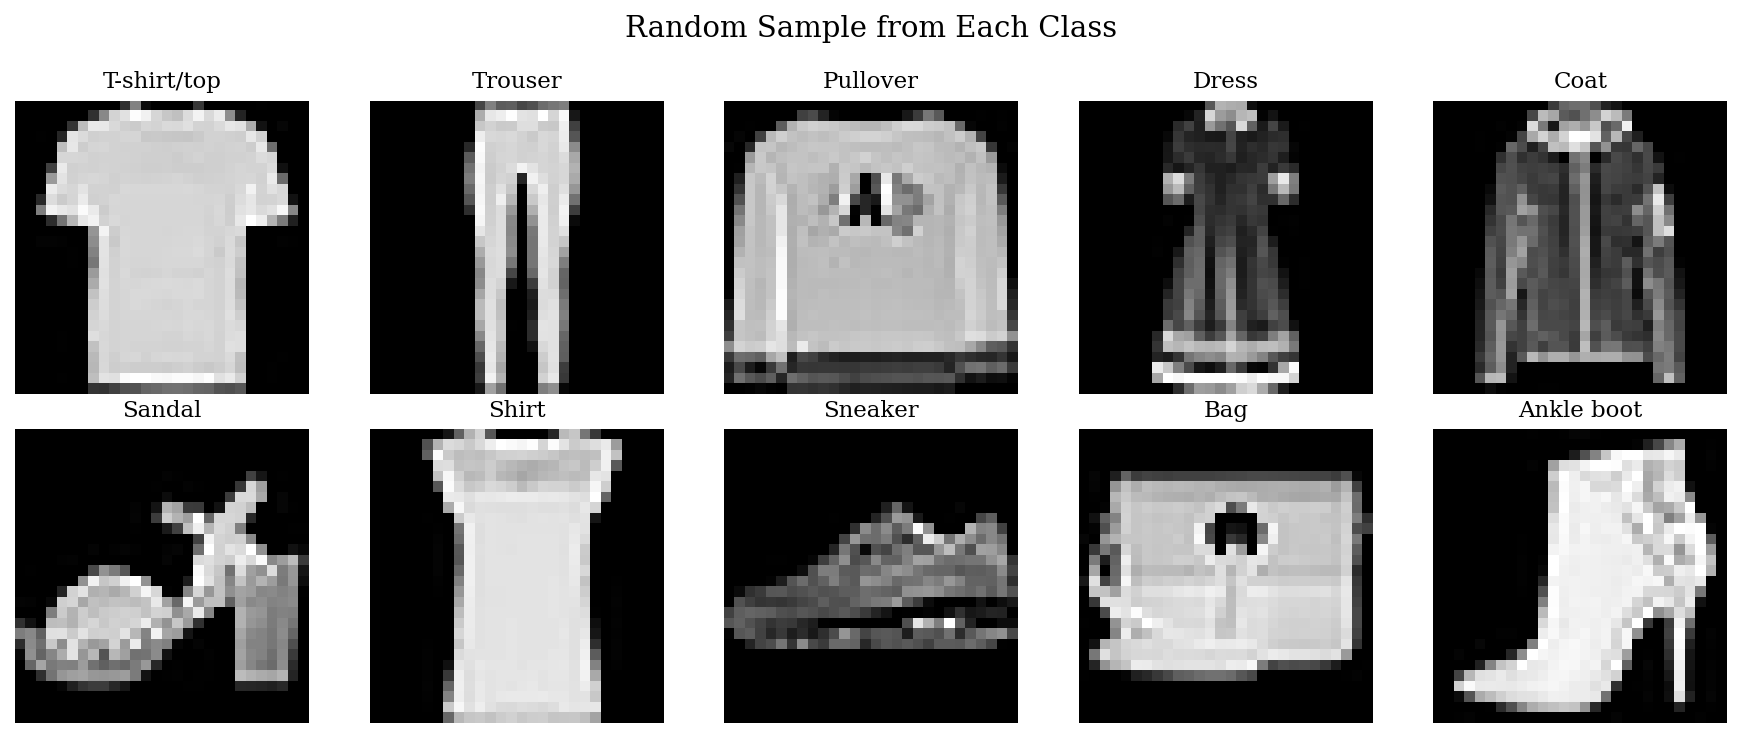
\includegraphics[width=0.85\textwidth]{figures/task1_samples.png}
	\caption{Random samples from each class in the Fashion MNIST training set. The visual similarity between T-shirt/Pullover/Coat/Shirt classes is evident.}
	\label{fig:samples}
\end{figure}

\begin{figure}[H]
	\centering
	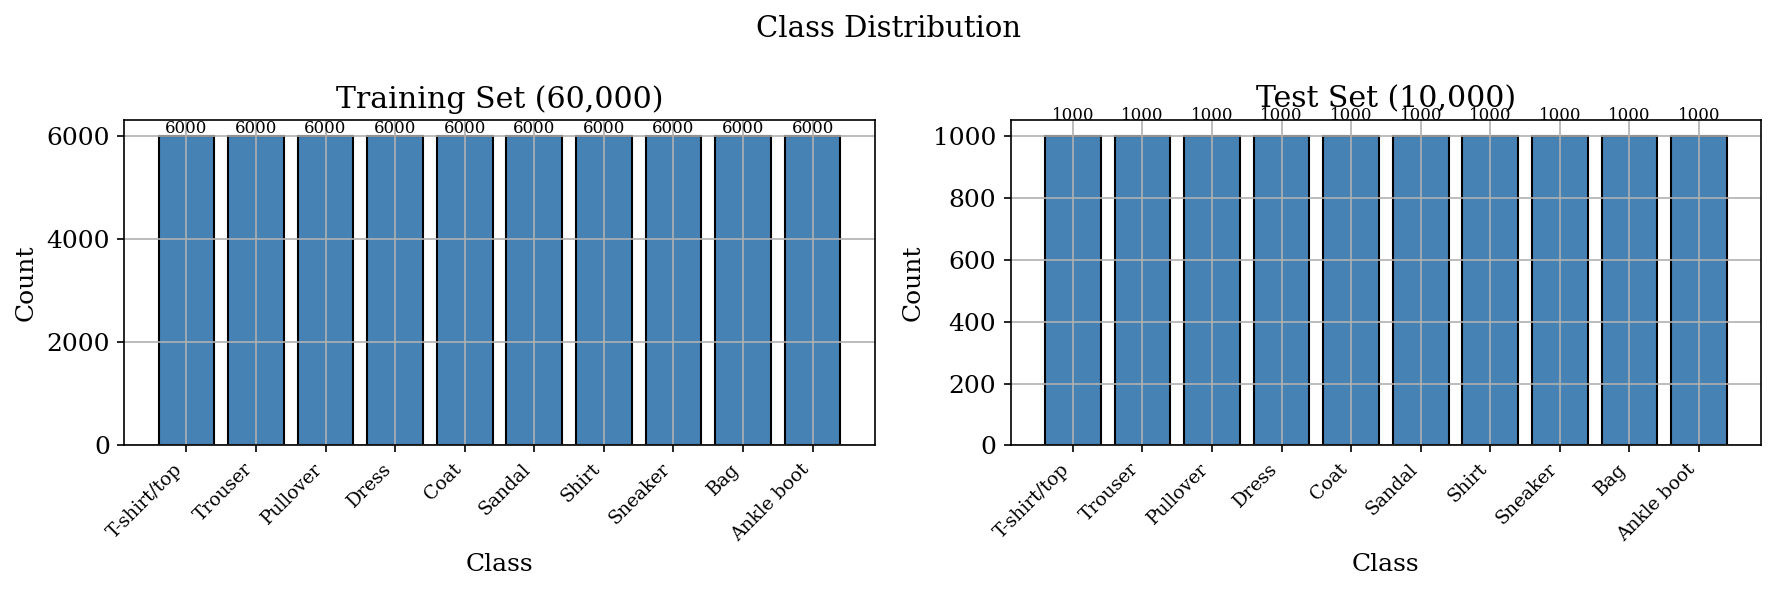
\includegraphics[width=0.7\textwidth]{figures/task1_class_distribution.png}
	\caption{Class distribution in training and test sets. Both sets are perfectly balanced with 6,000 and 1,000 samples per class respectively.}
	\label{fig:distribution}
\end{figure}

\begin{table}[H]
	\centering
	\caption{Dataset summary.}
	\begin{tabular}{lcc}
		\toprule
		Property                 & Training Set       & Test Set \\
		\midrule
		Samples                  & 60,000             & 10,000   \\
		Dimensions               & 784 (28$\times$28) & 784      \\
		Classes                  & 10                 & 10       \\
		Samples/class            & 6,000              & 1,000    \\
		Pixel range (raw)        & [0, 255]           & [0, 255] \\
		Pixel range (normalized) & [0, 1]             & [0, 1]   \\
		\bottomrule
	\end{tabular}
	\label{tab:data_summary}
\end{table}

Key observations from the EDA:
\begin{itemize}[nosep]
	\item The dataset is perfectly balanced, eliminating class imbalance as a confounding factor.
	\item Several classes are visually similar (T-shirt, Pullover, Coat, Shirt all have similar silhouettes), suggesting they will be harder to distinguish with pixel-level features.
	\item Footwear classes (Sandal, Sneaker, Ankle boot) and Bag have more distinctive shapes.
\end{itemize}

\subsection{Task 2: kNN Benchmark}

The 5-fold cross-validation over 28 hyperparameter combinations completed in approximately 36 minutes on 8 CPU cores.

\begin{table}[H]
	\centering
	\caption{Top 5 kNN hyperparameter combinations from 5-fold CV.}
	\begin{tabular}{cllcc}
		\toprule
		Rank & $k$        & Metric             & Weights           & Mean Acc $\pm$ Std           \\
		\midrule
		1    & \textbf{5} & \textbf{manhattan} & \textbf{distance} & \textbf{0.8625 $\pm$ 0.0033} \\
		2    & 7          & manhattan          & distance          & 0.8619 $\pm$ 0.0028          \\
		3    & 9          & manhattan          & distance          & 0.8616 $\pm$ 0.0030          \\
		4    & 3          & manhattan          & distance          & 0.8614 $\pm$ 0.0033          \\
		5    & 5          & manhattan          & uniform           & 0.8610 $\pm$ 0.0034          \\
		\bottomrule
	\end{tabular}
	\label{tab:knn_cv}
\end{table}

The best configuration ($k=5$, Manhattan distance, distance-weighted) achieves a test accuracy of \textbf{86.15\%}. The confusion matrix (Figure~\ref{fig:knn_cm}) reveals the expected pattern: upper-body clothing classes (T-shirt, Pullover, Coat, Shirt) are frequently confused with each other due to their similar silhouettes in pixel space.

\begin{figure}[H]
	\centering
	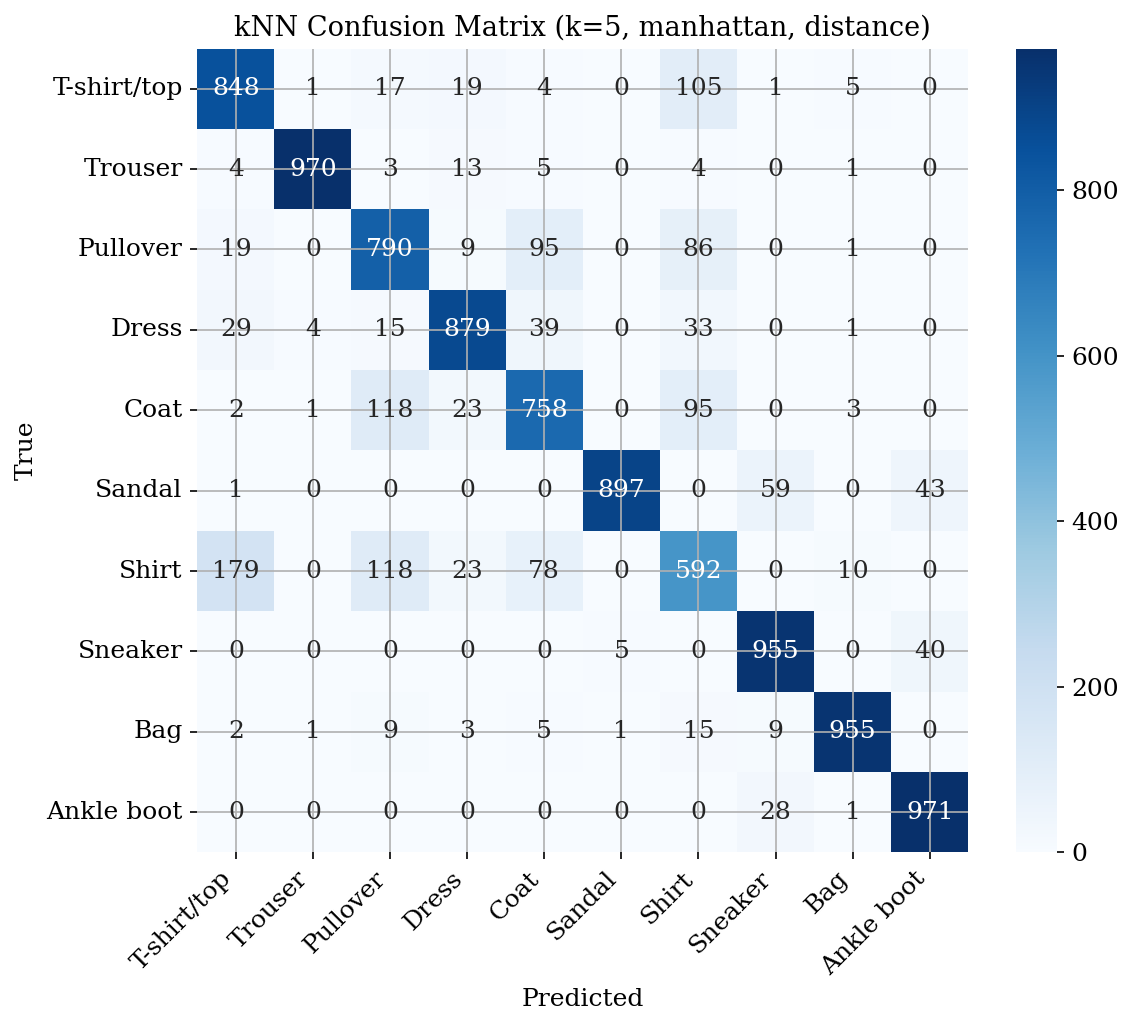
\includegraphics[width=0.5\textwidth]{figures/task2_knn_confusion_matrix.png}
	\caption{kNN confusion matrix on the test set. The ``Shirt'' class shows the most confusion, primarily with T-shirt, Pullover, and Coat.}
	\label{fig:knn_cm}
\end{figure}

\textbf{Discussion}: kNN operates directly on raw pixel distances. Two images of visually different items can have similar pixel distributions (e.g., a dark coat and a dark pullover), leading to misclassification. The method has no mechanism to learn invariant features --- it relies entirely on the chosen distance metric in the 784-dimensional input space.

\subsection{Task 3: PCA + kNN}

\begin{table}[H]
	\centering
	\caption{PCA + kNN results with varying number of components.}
	\begin{tabular}{cccc}
		\toprule
		Components   & Accuracy        & Runtime (s) & Variance Explained \\
		\midrule
		5            & 0.7359          & 14.7        & 0.6161             \\
		50           & 0.8638          & 18.3        & 0.8627             \\
		150          & \textbf{0.8708} & 29.3        & 0.9375             \\
		784 (no PCA) & 0.8615          & 62.2        & 1.0000             \\
		\bottomrule
	\end{tabular}
	\label{tab:pca_results}
\end{table}

\begin{figure}[H]
	\centering
	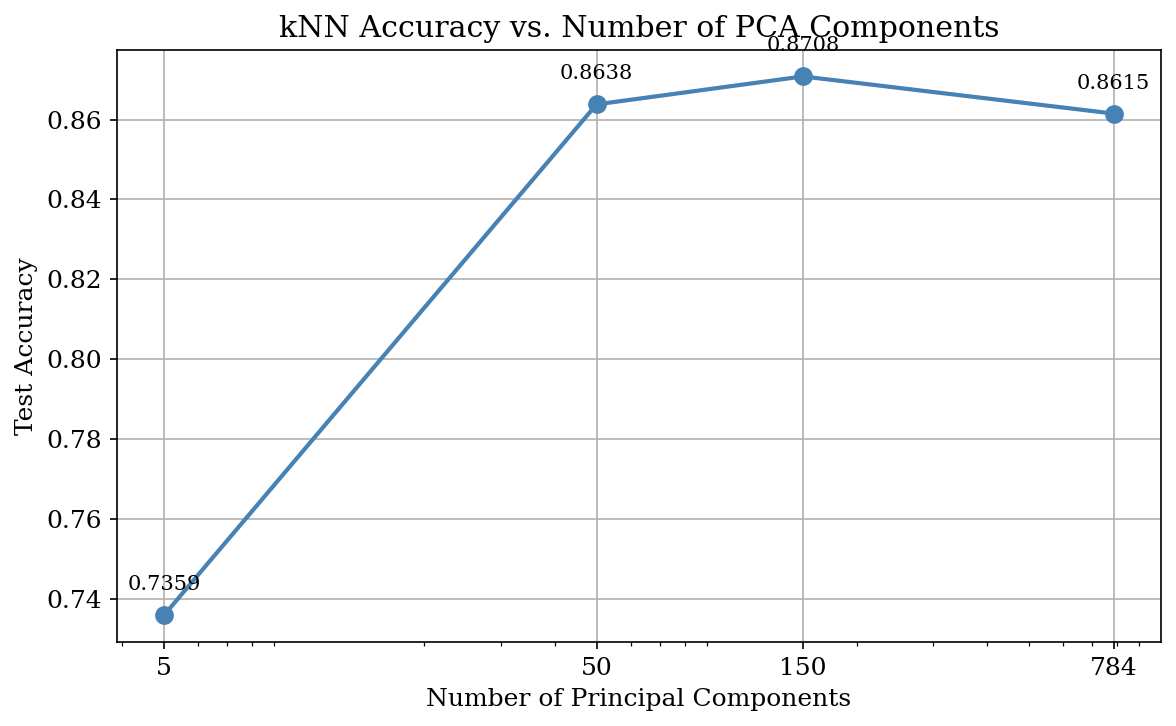
\includegraphics[width=0.7\textwidth]{figures/task3_accuracy_vs_components.png}
	\caption{kNN accuracy vs. number of PCA components. Accuracy peaks at 150 components, actually surpassing the full 784-dimensional baseline.}
	\label{fig:pca_acc}
\end{figure}

\begin{figure}[H]
	\centering
	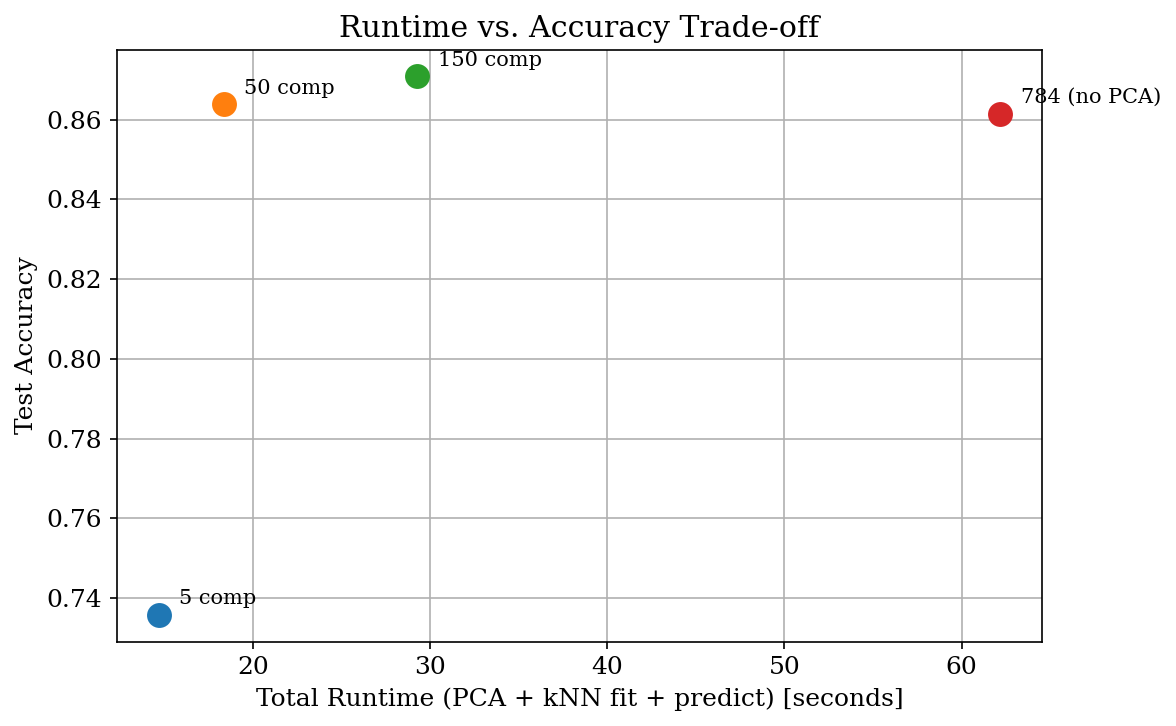
\includegraphics[width=0.7\textwidth]{figures/task3_runtime_vs_accuracy.png}
	\caption{Runtime vs. accuracy trade-off. PCA with 150 components achieves the best accuracy at half the runtime of the full-dimensional baseline.}
	\label{fig:pca_runtime}
\end{figure}

\textbf{Discussion}: A striking result is that PCA with 150 components (87.08\%) \emph{outperforms} the full 784-dimensional kNN (86.15\%). This demonstrates the \textbf{curse of dimensionality}: in high-dimensional spaces, distances become increasingly uniform, degrading kNN's discriminative ability. By projecting onto the top principal components, PCA removes noisy dimensions that contribute to distance computations but carry little class-relevant information, effectively improving the signal-to-noise ratio for distance-based classification. With 50 components (capturing 86.3\% of variance), kNN already matches full-dimensional performance at one-third the runtime. Extreme compression to 5 components (61.6\% variance) loses too much discriminative structure, dropping accuracy to 73.6\%.

\subsection{Task 4: Dense Neural Network}

\subsubsection{Model Selection Results}

\begin{table}[H]
	\centering
	\caption{Model selection results (80/20 validation split).}
	\begin{tabular}{lcc}
		\toprule
		Configuration       & Val Accuracy    & Early Stop Epoch \\
		\midrule
		A: [256, 128]       & 0.9042          & 45               \\
		B: [512, 256]       & 0.9045          & 36               \\
		C: [512, 256, 128]  & \textbf{0.9100} & 49               \\
		D: [1024, 512, 256] & 0.9072          & 46               \\
		\bottomrule
	\end{tabular}
	\label{tab:nn_selection}
\end{table}

\begin{figure}[H]
	\centering
	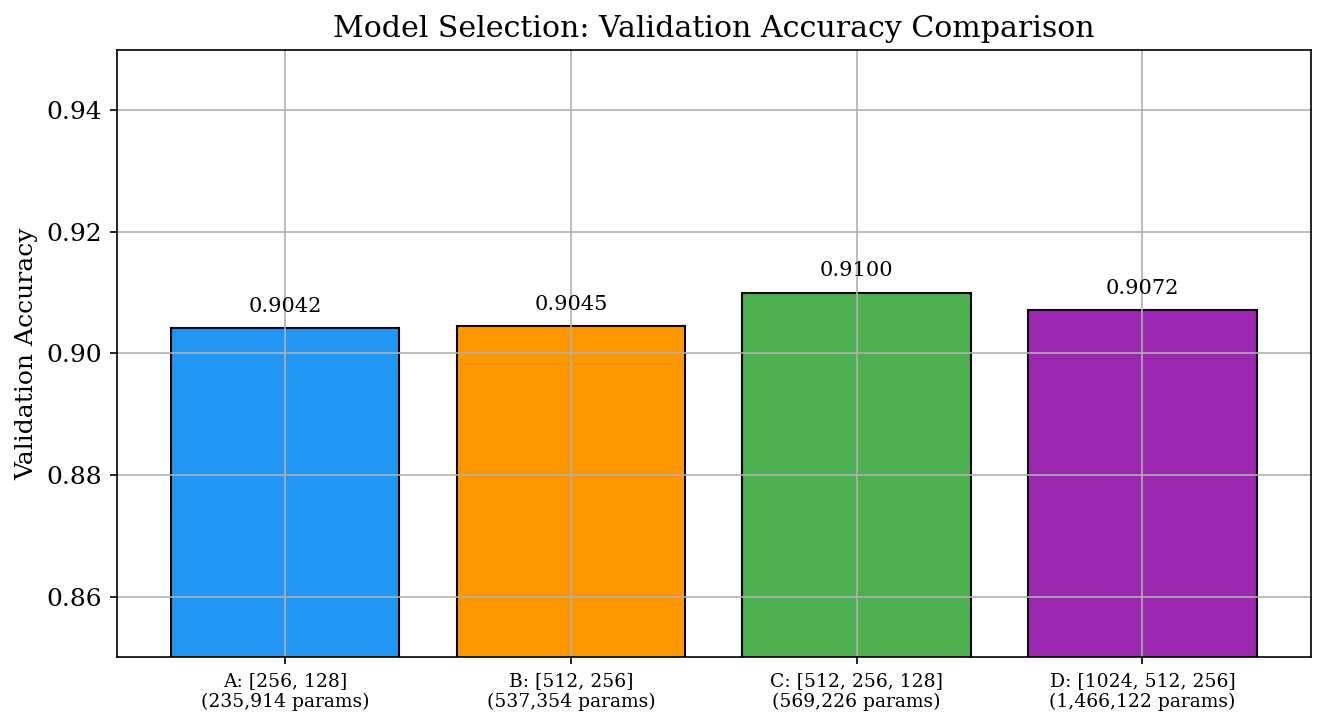
\includegraphics[width=0.75\textwidth]{figures/task4_model_selection.png}
	\caption{Validation accuracy comparison across the four configurations. Config C achieves the highest validation accuracy.}
	\label{fig:model_selection}
\end{figure}

Config C ([512, 256, 128] with dropout 0.4) was selected with 91.00\% validation accuracy. The deeper architecture with stronger regularization outperforms both wider-but-shallower (Config B) and larger (Config D) alternatives. This illustrates the bias--variance tradeoff: Config D has more capacity but its additional parameters do not translate to better performance given the regularization and data size, while the extra hidden layer in Config C provides hierarchical feature extraction that the two-layer architectures lack.

\subsubsection{Final Model Performance}

After retraining on 90\% of the training data (54,000 samples) with 10\% held out for early stopping:

\begin{figure}[H]
	\centering
	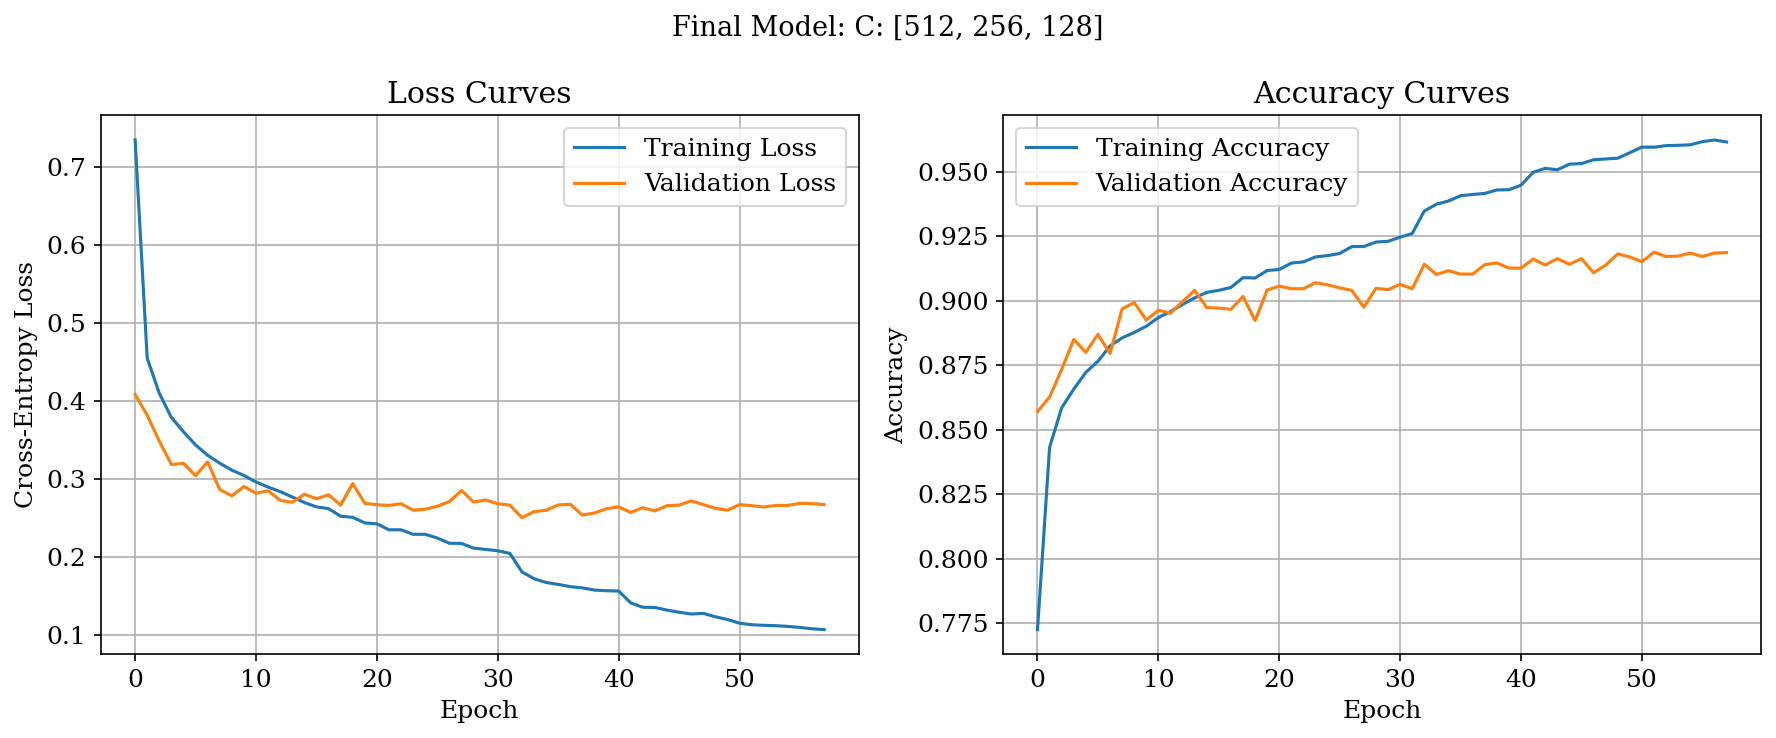
\includegraphics[width=0.85\textwidth]{figures/task4_training_curves.png}
	\caption{Training and validation loss/accuracy curves for the final model (Config C). Smooth convergence with minimal overfitting gap.}
	\label{fig:training_curves}
\end{figure}

\begin{figure}[H]
	\centering
	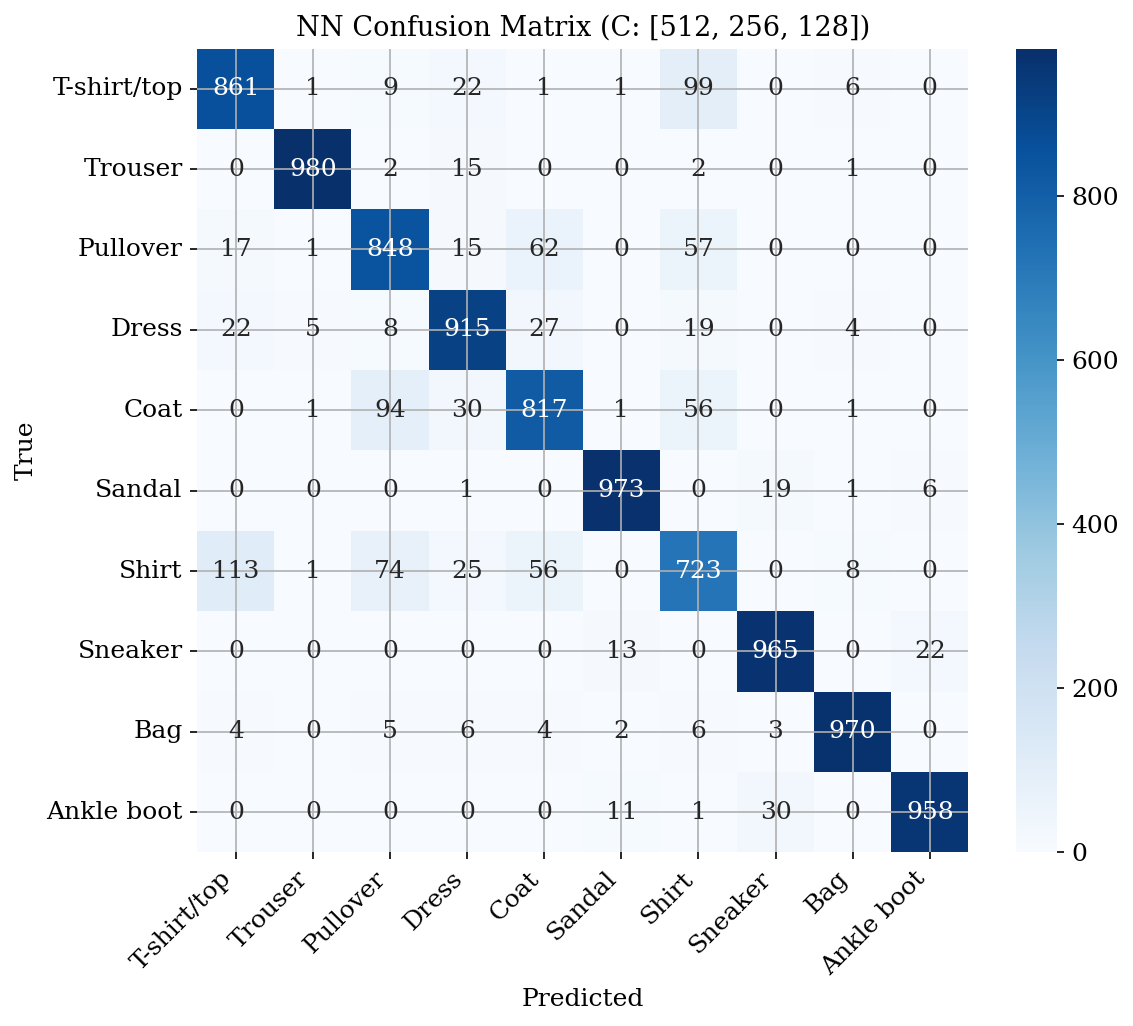
\includegraphics[width=0.5\textwidth]{figures/task4_nn_confusion_matrix.png}
	\caption{Neural network confusion matrix on the test set. The NN significantly reduces confusion among upper-body classes compared to kNN.}
	\label{fig:nn_cm}
\end{figure}

\begin{table}[H]
	\centering
	\caption{Per-class accuracy for the neural network.}
	\begin{tabular}{lc}
		\toprule
		Class       & Accuracy \\
		\midrule
		T-shirt/top & 0.8700   \\
		Trouser     & 0.9860   \\
		Pullover    & 0.8480   \\
		Dress       & 0.9150   \\
		Coat        & 0.8170   \\
		Sandal      & 0.9730   \\
		Shirt       & 0.7230   \\
		Sneaker     & 0.9650   \\
		Bag         & 0.9700   \\
		Ankle boot  & 0.9580   \\
		\bottomrule
	\end{tabular}
	\label{tab:nn_per_class}
\end{table}

The Shirt class remains the hardest (72.3\% accuracy), consistently confused with T-shirt, Pullover, and Coat. These classes share similar global structure (rectangular torso shape with sleeve-like extensions). The neural network, despite learning non-linear feature combinations, still struggles because the distinguishing features (collar type, sleeve length, texture patterns) require spatial awareness that a fully connected network operating on flattened pixels cannot fully exploit.

\subsection{Task 5: Comparative Analysis}

\begin{table}[H]
	\centering
	\caption{Final comparison: kNN vs. Dense Neural Network on the test set.}
	\begin{tabular}{lcc}
		\toprule
		Metric               & kNN    & Dense NN \\
		\midrule
		Accuracy             & 0.8615 & 0.9010   \\
		Precision (weighted) & 0.8627 & 0.9009   \\
		Recall (weighted)    & 0.8615 & 0.9010   \\
		\bottomrule
	\end{tabular}
	\label{tab:comparison}
\end{table}

\begin{figure}[H]
	\centering
	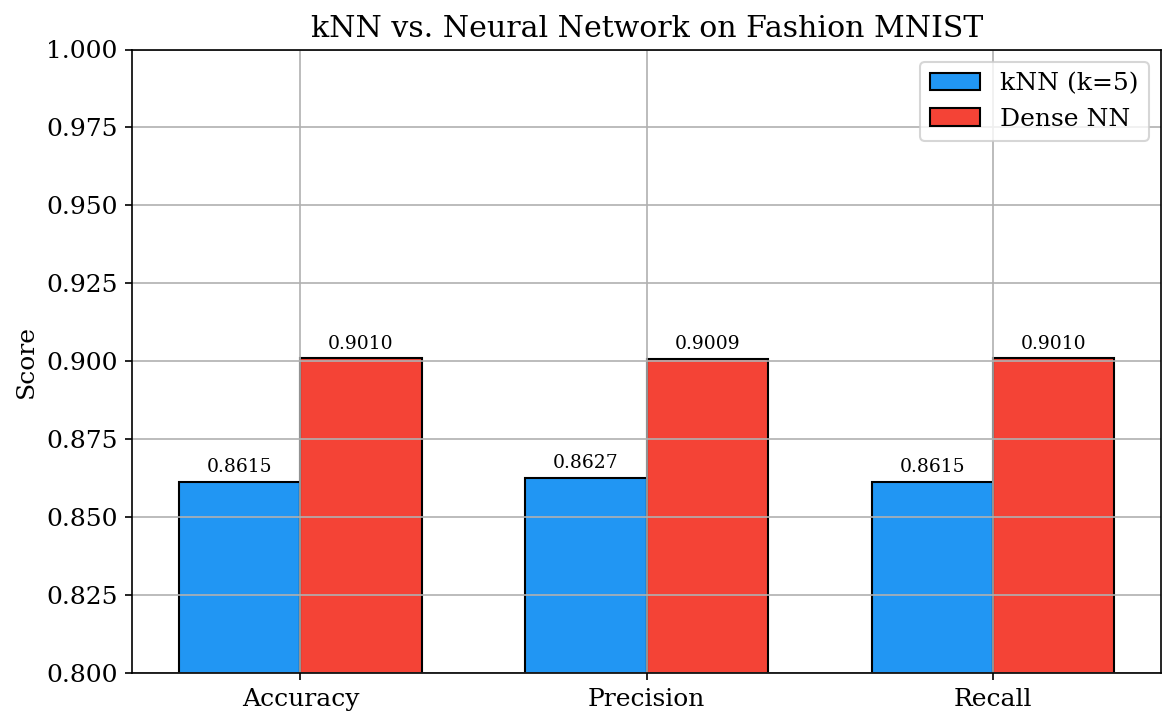
\includegraphics[width=0.7\textwidth]{figures/task5_comparison.png}
	\caption{Overall metrics comparison between kNN and the dense neural network.}
	\label{fig:comparison}
\end{figure}

\begin{figure}[H]
	\centering
	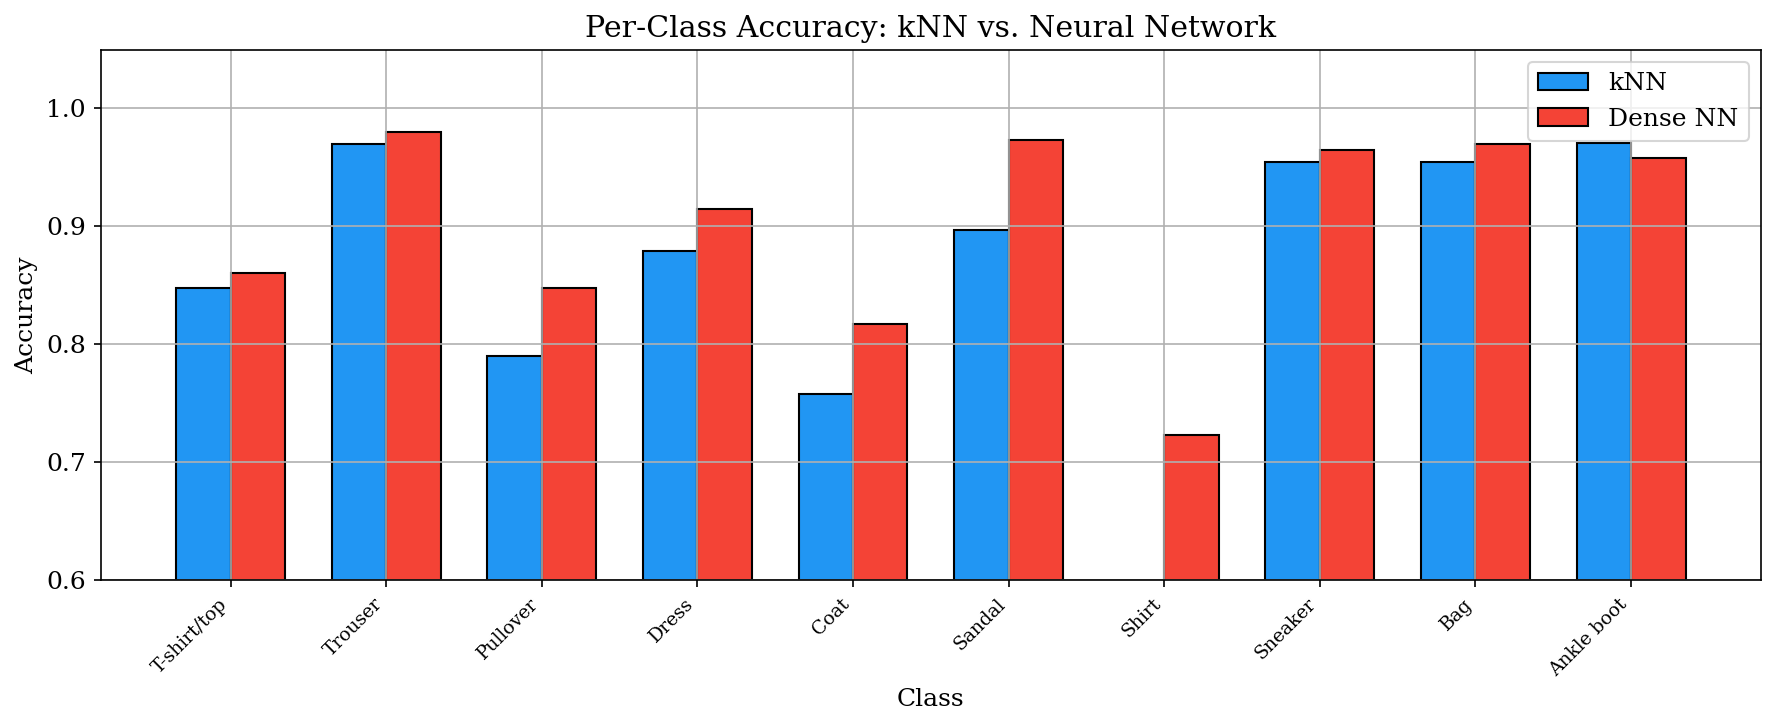
\includegraphics[width=0.85\textwidth]{figures/task5_per_class_comparison.png}
	\caption{Per-class accuracy comparison. The NN consistently outperforms kNN, with the largest gains on difficult classes.}
	\label{fig:per_class}
\end{figure}

\textbf{Key findings}:
\begin{enumerate}[nosep]
	\item \textbf{Neural network outperforms kNN}: The dense NN achieves higher accuracy across all metrics, demonstrating the value of learned representations over raw pixel distances.
	\item \textbf{Largest gains on difficult classes}: The NN's advantage is most pronounced for classes like Shirt, Coat, and Pullover where pixel-level similarity is misleading.
	\item \textbf{kNN strengths}: Requires no training phase (lazy learner), easily interpretable through nearest neighbor visualization, and competitive on ``easy'' classes with distinctive shapes.
	\item \textbf{NN strengths}: Learns non-linear decision boundaries and hierarchical features; fast inference after training; scales better with data.
	\item \textbf{Both struggle with}: The Shirt class, which shares visual features with multiple other upper-body categories.
\end{enumerate}

\textbf{Why does the NN win?} kNN computes distances in the raw 784-dimensional pixel space. In this space, semantically different images can be close (e.g., a black coat and a black pullover) while semantically similar images can be far (e.g., a white vs.\ black T-shirt). The neural network's hidden layers learn to map raw pixels into a feature space where class boundaries are more separable --- a form of automatic feature engineering that kNN cannot perform.

\textbf{Suggested improvement}: A Convolutional Neural Network (CNN) would exploit the 2D spatial structure of images, learning translation-invariant features (edges, textures, patterns) that are crucial for distinguishing upper-body clothing categories. Data augmentation (random translations, horizontal flips) would further improve generalization.

\section{Conclusion}

We compared k-Nearest Neighbors and dense neural networks on Fashion MNIST classification. The dense neural network (3-layer, [512, 256, 128] architecture with dropout 0.4) achieves superior accuracy over the best kNN configuration, confirming that learned representations outperform raw pixel distances for image classification.

Key takeaways:
\begin{itemize}[nosep]
	\item kNN provides a strong non-parametric baseline but is limited by operating in raw pixel space.
	\item PCA dimensionality reduction can maintain kNN accuracy while significantly reducing computation, confirming the low effective dimensionality of the data.
	\item Dense neural networks learn hierarchical features through non-linear transformations, yielding better class separation.
	\item Model selection via validation error minimization identified that a 3-layer architecture with strong regularization (dropout 0.4) optimally balances capacity and generalization.
	\item The remaining classification errors concentrate on visually similar upper-body clothing classes, suggesting that spatial feature extraction (CNNs) is needed for further improvement.
\end{itemize}

\begin{thebibliography}{9}
	\bibitem{xiao2017} Xiao, H., Rasul, K., \& Vollgraf, R. (2017). Fashion-MNIST: a Novel Image Dataset for Benchmarking Machine Learning Algorithms. arXiv:1708.07747.
\end{thebibliography}

\end{document}
